%% 
%% Copyright 2019-2021 Elsevier Ltd
%% 
%% This file is part of the 'CAS Bundle'.
%% --------------------------------------
%% 
%% It may be distributed under the conditions of the LaTeX Project Public
%% License, either version 1.2 of this license or (at your option) any
%% later version.  The latest version of this license is in
%%    http://www.latex-project.org/lppl.txt
%% and version 1.2 or later is part of all distributions of LaTeX
%% version 1999/12/01 or later.
%% 
%% The list of all files belonging to the 'CAS Bundle' is
%% given in the file `manifest.txt'.
%% 
%% Template article for cas-sc documentclass for 
%% single column output.

\documentclass[a4paper,fleqn]{cas-sc}

% If the frontmatter runs over more than one page
% use the longmktitle option.
%\documentclass[a4paper,fleqn,longmktitle]{cas-sc}

%\usepackage[numbers]{natbib}
\usepackage[authoryear]{natbib}
%\usepackage[authoryear,longnamesfirst]{natbib}



%%=====
%%=====  Packages included by us
%%=====
% Took this part from elsarticle example
\usepackage[mathlines]{lineno} 
\modulolinenumbers[1]

\usepackage{anyfontsize}
\usepackage{lipsum}
\usepackage{xcolor} 
\usepackage{csquotes} % In order to use \enquote
\usepackage{float}
\usepackage{textcomp}
\usepackage{relsize} % In order to use \mathsmaller
\usepackage{upgreek} % Need extra font for greek letters
\usepackage[section]{placeins} % Keep figures within same section
\usepackage{tabularx} % Table with automatic line break within a cell
\usepackage{caption}
\usepackage{hyperref} 
\usepackage{afterpage}

% I wanted amsfonts for mathbb (i.e. with serif), not the one included in cas-sc
\DeclareSymbolFontAlphabet{\mathbb}{AMSb}

% Same thing for mathcal
\DeclareSymbolFont{cmsymbols}{OMS}{cmsy}{m}{n}
\SetSymbolFont{cmsymbols}{bold}{OMS}{cmsy}{b}{n}
\DeclareSymbolFontAlphabet{\mathcal}{cmsymbols}

% Hyperbolyc secant was missing
\DeclareMathOperator{\sech}{sech}

% Override \vec with an invocation of \vect.
\newcommand{\vect}[1]{\boldsymbol{\mathbf{#1}}}

\let\stdvec\vec
\renewcommand{\vec}[1]{\vect{#1}}

% ---- Change the real and imaginary symbols to something that looks nicer (in our opinion)
\renewcommand{\Re}{\operatorname{Re}}
\renewcommand{\Im}{\operatorname{Im}}

% In order to make smaller subscripts. For instance, $\varphi_O$ was too big
\newcommand{\sbs}[1]{_{\!\mathsmaller{#1}}}

% Useful for some tables
\newcolumntype{Y}{>{\centering\arraybackslash}X}


%%%% Solution found at
%%%% https://tex.stackexchange.com/questions/436011/linenomath-printing-extra-numbers-on-last-line-of-multline-align-flalign-envir
%%%% for the problem of numbering nested equations
\usepackage{etoolbox} %% <- for \cspreto, \csappto, \patchcmd, \pretocmd, \apptocmd

%% Patch 'normal' math environments:
\newcommand*\linenomathpatch[1]{%
  \cspreto{#1}{\linenomath}%
  \cspreto{#1*}{\linenomath}%
  \csappto{end#1}{\endlinenomath}%
  \csappto{end#1*}{\endlinenomath}%
}

%% Patch AMS math environments:
\newcommand*\linenomathpatchAMS[1]{%
  \cspreto{#1}{\linenomathAMS}%
  \cspreto{#1*}{\linenomathAMS}%
  \csappto{end#1}{\endlinenomath}%
  \csappto{end#1*}{\endlinenomath}%
}

%% Definition of \linenomathAMS depends on whether the mathlines option is provided
\expandafter\ifx\linenomath\linenomathWithnumbers
  \let\linenomathAMS\linenomathWithnumbers
  %% The following line gets rid of an extra line numbers at the bottom:
  \patchcmd\linenomathAMS{\advance\postdisplaypenalty\linenopenalty}{}{}{}
\else
  \let\linenomathAMS\linenomathNonumbers
\fi

\linenomathpatch{equation}
\linenomathpatchAMS{gather}
\linenomathpatchAMS{multline}
\linenomathpatchAMS{align}
\linenomathpatchAMS{alignat}
\linenomathpatchAMS{flalign}


% This essentially duplicates \substack, but adding an alignment point.
\makeatletter
\newcommand{\subalign}[1]{%
  \vcenter{%
    \Let@ \restore@math@cr \default@tag
    \baselineskip\fontdimen10 \scriptfont\tw@
    \advance\baselineskip\fontdimen12 \scriptfont\tw@
    \lineskip\thr@@\fontdimen8 \scriptfont\thr@@
    \lineskiplimit\lineskip
    \ialign{\hfil$\m@th\scriptstyle##$&$\m@th\scriptstyle{}##$\hfil\crcr
      #1\crcr
    }%
  }%
}
\makeatother


% Keep floats inside subsection
\let\Oldsection\section
\renewcommand{\section}{\FloatBarrier\Oldsection}

\let\Oldsubsection\subsection
\renewcommand{\subsection}{\FloatBarrier\Oldsubsection}

%%=====
%====== END OF MY MODIFICATIONS
%%=====



\begin{document}
\let\WriteBookmarks\relax
\def\floatpagepagefraction{1}
\def\textpagefraction{.001}

% Short title
\shorttitle{Discussion on some relevant aspects for the experimental and numerical analysis of FWTs}

% Short author
\shortauthors{L. H. S. do Carmo, P. C. de Mello, R. M. Monaro and A. N. Simos}

% Main title of the paper
\title [mode = title]{A discussion on some relevant aspects for the experimental and numerical analysis of floating wind turbines based on a test case}

% Title footnote mark
% eg: \tnotemark[1]
%\tnotemark[<tnote number>] 

% Title footnote 1.
% eg: \tnotetext[1]{Title footnote text}
%\tnotetext[<tnote number>]{<tnote text>} 

% First author
%
% Options: Use if required
% eg: \author[1,3]{Author Name}[type=editor,
%       style=chinese,
%       auid=000,
%       bioid=1,
%       prefix=Sir,
%       orcid=0000-0000-0000-0000,
%       facebook=<facebook id>,
%       twitter=<twitter id>,
%       linkedin=<linkedin id>,
%       gplus=<gplus id>]
\author[1]{Lucas H. S. do Carmo}[orcid=0000-0001-8744-1391]

% Corresponding author indication
\cormark[1]
\cortext[1]{Corresponding author.}

% Footnote of the first author
%\fnmark[1]

% Email id of the first author
\ead{lucas.carmo@usp.br}

% URL of the first author
%\ead[url]{lucas.carmo@usp.br}

% Credit authorship
\credit{Conceptualization, Methodology, Software, Validation, Formal analysis, Writing -- original draft}

% Address/affiliation
\affiliation[1]{organization={University of São Paulo},
            addressline={Av. Prof. Mello Moraes, 2231}, 
            city={São Paulo},
            %citysep={}, % Uncomment if no comma needed between city and postcode
            postcode={05508-030}, 
            %state={SP},
            country={Brazil}}

\author[1]{Pedro C. de Mello}[orcid=0000-0003-2621-9644]
\credit{Conceptualization, Experiments}
\author[1]{Renato M. Monaro}[orcid=0000-0002-7453-8650]
\credit{Conceptualization, Experiments}
\author[1]{Alexandre N. Simos}[orcid=0000-0002-1879-5468]
\credit{Conceptualization, Formal analysis, Writing -- review, Supervision}



% For a title note without a number/mark
%\nonumnote{}

% Here goes the abstract
\begin{abstract}
A \lipsum[1-1]
\end{abstract}

% Keywords
% Each keyword is seperated by \sep
\begin{keywords}
    \sep Floating wind turbines \sep Model tests \sep Numerical modeling \sep Software-in-the-loop
\end{keywords}
  
\maketitle

% Main text
\linenumbers
\section{Introduction} \label{sec:introduction}
Floating offshore wind turbines (FOWTs) have been the subject of numerous studies due to the possibility of exploiting the vast wind resources located in deep waters. As an emerging technology, the growth of the wind energy industry depends on FOWTs achieving more competitive costs, which has pushed for larger rotors and new designs for both floaters and moorings.

Since FOWTs are complex structures, their design requires the evaluation of performance and structural integrity for a myriad of environmental conditions (wind, wave, current, among others) and operating conditions (power production, normal shut down, fault conditions, etc.). Due to their intricate dynamics, this procedure requires modeling software capable of accounting for the couplings between aerodynamics, hydrodynamics, controls, moorings and structural behavior, which are commonly referred as aero-hydro-servo-elastic tools. A substantial effort has been made to validate these software, as exemplified by the OC3~\citep{jonkman2010report}, OC4~\citep{OC42014} and OC5~\citep{OC52017} projects, but this is still an ongoing development.

In fact, the experiments required to validate the numerical tools, usually performed in model scale, are far from an easy task, for it is impossible to keep all the dimensionless parameters that describe the different physical aspects of the problem. For instance, while the scaling of the waves requires that the Froude number ($\textrm{Fr} = U^{2}/(gL)$, with $U$ a characteristic speed, $L$ a characteristic length and $g$ the gravitational acceleration) be conserved, the aerodynamic loads are governed by the Reynolds number ($\textrm{Re} = UL/\nu$, with $\nu$ the kinematic viscosity). To work around this incompatibility, some alternatives have been tried to perform tests with both wind and waves, and a thorough review of experimental techniques for doing so can be found in \citet{otter2022review}. For instance, some works have used a Froude scaled rotor with  the wind generated by fans at higher speeds than the scaled ones, so that the correct rotor thrust was obtained \citep{martin2014methodology, skaare2007integrated, mortensen2018experimental}; however, this approach has the downside that either the tip speed ratio (TSR) or the excitation frequencies are not preserved. Others have employed performance scaled rotors \citep{goupee2014experimental, de2014development, bredmose2017triple}, in the sense that the rotors were redesigned with geometrically modified airfoils to compensate for the low Reynolds number obtained in a Froude scale experiment. 

A different line of thought is adopted by the so-called hybrid tests, in which either the aerodynamic or hydrodynamic forces are computed numerically and applied to the FOWT instead of being a consequence of the physical interaction of the hull/rotor with the waves/wind. The present work deals with the case in which the experiments are performed in a wave basin, so the waves are still generated physically, while the aerodynamic forces are replaced by a numerical model. This approach, called software-in-the-loop (SIL), was first employed by \citet{azcona2014aerodynamic}, who used a single ducted propeller in place of the turbine rotor to emulate the aerodynamic thrust, while the aerodynamic forces acting on the other degrees of freedom were disregarded. In a nutshell, it consists in measuring the motions of the FOWT model, which is floating in the wave basin, and feeding these motions to the software, in which the aerodynamic forces acting on a virtual rotor under the action of a virtual wind are computed numerically -- in that case and in the present work, using Blade Element Momentum Theory (BEMT). Finally, the rotational speed of the fan is controlled in order to provide the required thrust. The fact that this procedure happens in real time and taking into account the motions of the structure makes it simple to synchronize wave elevation and wind loads, besides allowing the modeling of aerodynamic damping and turbine control. In subsequent works, the SIL method has been applied with multi-propeller actuators in order to model not only the aerodynamic thrust, but also the forces and moments along the other degrees of freedom \citep{pires2020inclusion, otter2020emulating}. 

Alternatively, some works have employed cables pulled by winches instead of fans to emulate the aerodynamic loads \citep{sauder2016real, bachynski2016real, thys2018real}, while the option of performing the experiment in a wind tunnel whilst the hydrodynamics of the FOWT is computed numerically is discussed by \citet{bayati2018wind} and \citet{belloli2020hybrid}. However, the SIL method proposed by \citet{azcona2014aerodynamic} has the advantage of being the simplest option in terms of required equipment for a wave basin such as the one from the Numerical Offshore Tank of the University of São Paulo (TPN-USP). 

Besides improving the capabilities of TPN-USP to be able to perform experimental tests of FOWTs under the concomitant action of wind and waves, this work aims at validating the numerical models that were used during the design of a FOWT concept (illustrated in Figure~\textcolor{red}{1}) developed in the context of a joint research project with Petrobras~\citep{mas2022parametric}. Due to these two different objectives, this paper is divided in two parts:
\begin{enumerate}[i.]
    \item In the first part, which is provided in Section~\ref{sec:exp_vs_num}, the experiments are used to verify aspects of the hydrodynamics of the floater (which is the part that is physically present in the tests) that the numerical models should take into account. More specifically, a numerical model as close as possible to the conditions of the experiment is built using OpenFAST~\cite{jonkman2005fast} and WAMIT~\cite{wamitManual}, and this model is used to assess the importance of drag forces on the pontoons and of second-order wave forces in both the horizontal and vertical degrees of freedom (dofs). It is also shown that the mean hull inclination due to the wind is not much relevant for the computation of radiation/diffraction coefficients;
%%%%%%%%%%%%%%%%
    \item In the second part, described in Section~\ref{sec:impact_simplifications}, the objective is to investigate the relevance of two physical aspects that were not included in the aerodynamic modeling adopted in the tests. The first of them is that the SIL implementation employed a fan assembly that was only able to apply the aerodynamic thrust, thus loads in the other dofs were not present in the model; the other aspect is that blade elasticity was not considered in this first version of the software, a point that is planned to be addressed in future versions. In order to verify the impact of these simplifications, the numerical models that are discussed in the first part of the paper are compared with additional OpenFAST models that include both blade elasticity and the aerodynamic forces on the six dofs.
% (embora de forma simples com o elastodyn. Preciso estudar em que situações seria necessário usar o beamdyn).
\end{enumerate}

after describing the prototype and experimental setup in Section~\ref{sec:description_experiment} and the numerical models that were 

including the limitations of the SIL approach implemented


Explicar nosso objetivo, que é duplo: verificar nossos modelos numéricos e, concomitantemente, desenvolver a capacidade do tanque de provas numérico em realizar esse tipo de ensaio.

Ensaio com SIL com algumas limitações

\section{Description of the prototype and the experimental setup} \label{sec:description_experiment}
The FOWTC hull concept is the result of the parametrical optimization procedure reported by \citet{mas2022parametric}. Following the two objectives given in Section~\ref{sec:introduction}, the experiments were conducted in such a way that they were as close as possible to the design conditions in order to allow for the verification of the numerical methods. Two main differences are, however, present: the water depth, which had to be reduced from $600\,\text{m}$ to $233\,\text{m}$, and the limitations of the software-in-the-loop approach, outlined in Section~\ref{sec:introduction} and discussed in details in Section~\ref{sec:impact_simplifications}.

The experimental campaign was conducted at the wave basin of the Numerical Offshore Tank of the University of São Paulo (TPN-USP), a squared $14\,\text{m}\times 14\,\text{m} \times 4\,\text{m}$ (length, width, depth) tank equipped with 152 active-absorption flap-type wave generators that is shown in Figure~\ref{fig:description_experiment:tanque}.
\begin{figure}[!hbtp]
	\centering
	\includegraphics[width=0.5\columnwidth]{./figures/CH-tpn.jpg}%
	\caption{Wave basin of the Numerical Offshore Tank of the University of São Paulo.} \label{fig:description_experiment:tanque}%
\end{figure}%


\subsection{Main properties of the FOWTC}
%- Caracteristicas da FOWT, RNA, ancoragem
The FOWTC concept consists of a semi-submersible hull with a $14.1\,\text{m}$ diameter central column attached to three $17.0\,\text{m}$ diameter columns arranged as an equilateral triangle, connected by rectangular pontoons $17.0\,\text{m}$ high and $6.0\,\text{m}$ wide, which was built in a 1:70 scale for the experiments. 

During design, the RNA of the IEA 15MW turbine \citep{gaertner2020definition} and the tower of the UMaine VolturnUS-S floater~\citep{allen2020definition} were mounted on top of the central column, but their inertial and structural characteristics were not preserved during the tests. Instead, the global inertial properties of the whole FOWT were matched by using a ballast system that included a moving set of weights that could be adjusted along a fuse located on top of the tower. A picture of the model is given in Figure~\ref{fig:description_experiment:modelo}, while its main properties are listed in Table~\ref{tab:description_experiment:FOWTC_properties}.
\begin{figure}[!hbtp]
	\centering
	\includegraphics[height=10cm]{./figures/foto_modelo.png}%
	\caption{Picture of the FOWTC model.} \label{fig:description_experiment:modelo}%
\end{figure}%
%\begin{figure}[!hbtp]
%	\centering
%	\fbox{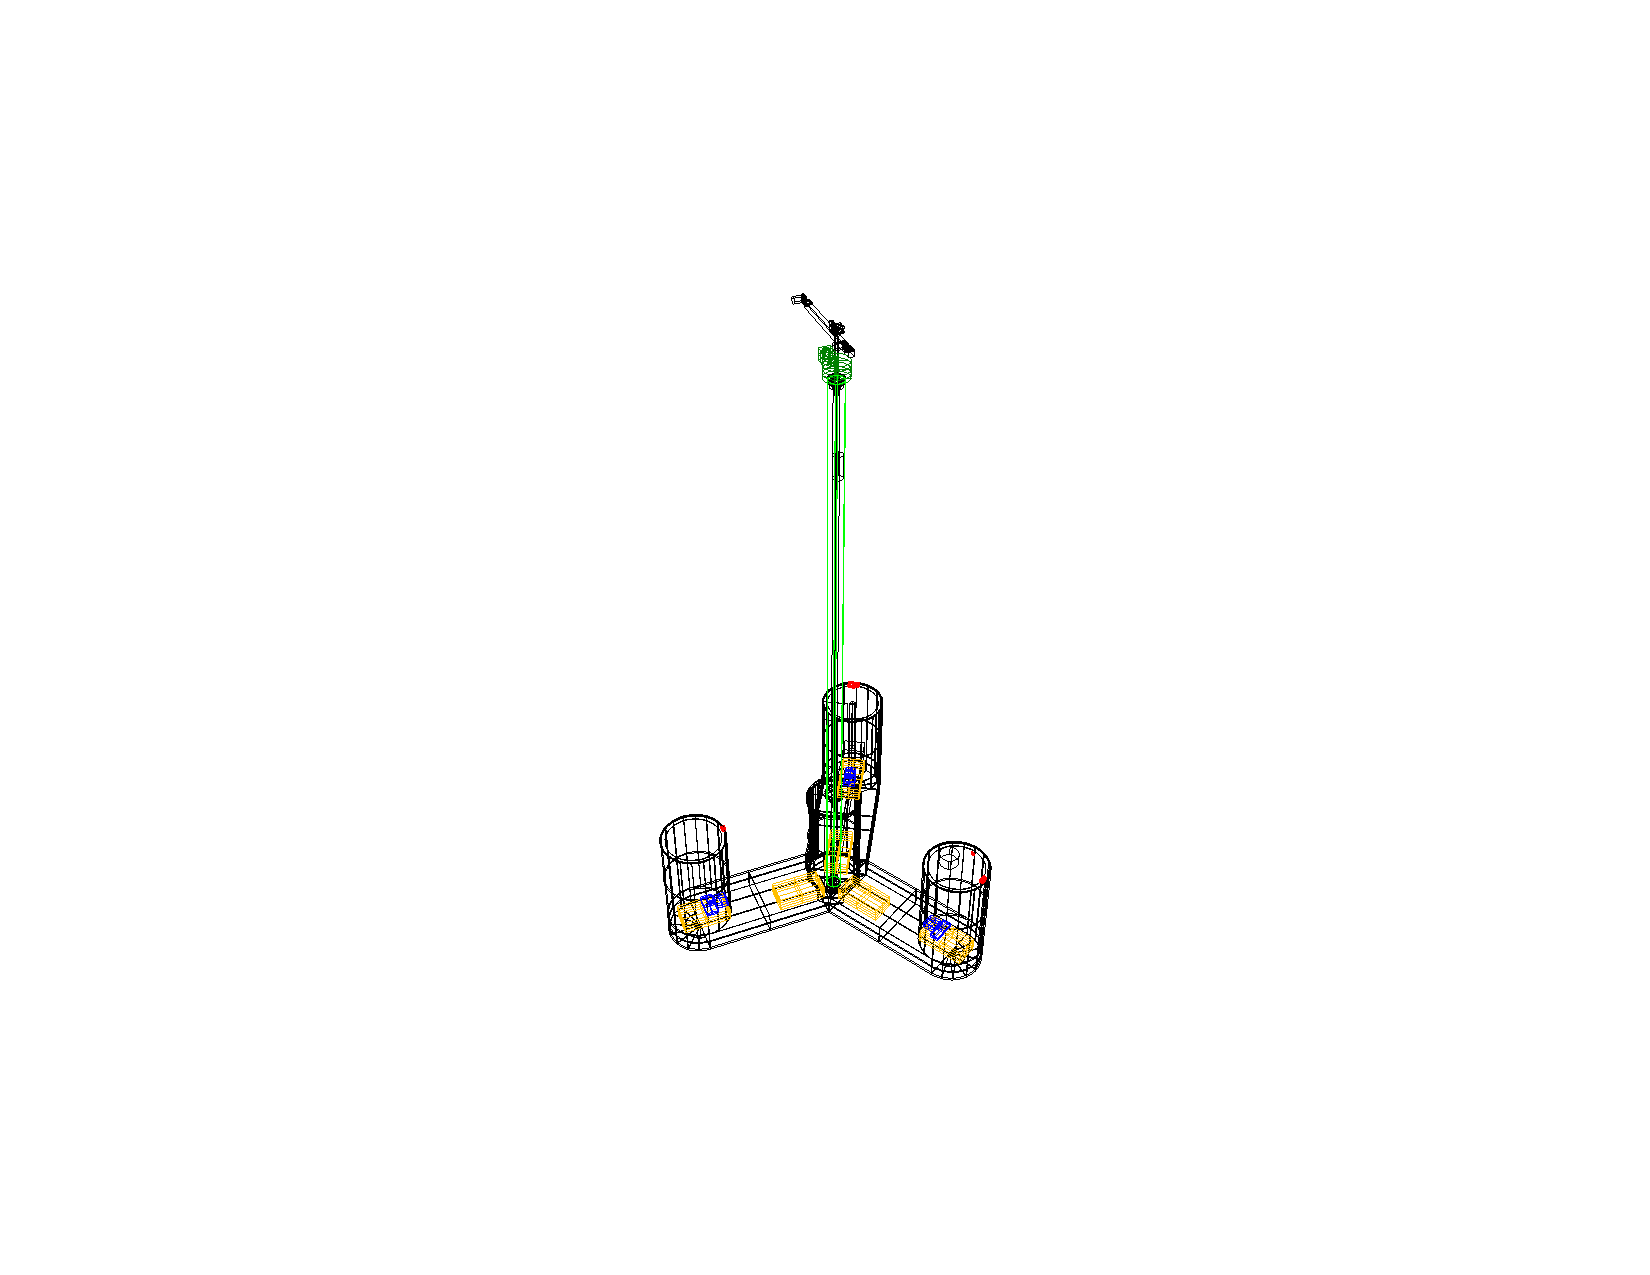
\includegraphics[trim={11cm 5cm 11cm 5cm},clip, height=10cm]{./figures/rhino_lastros.pdf}}%
%	\caption{Picture of the FOWTC model.} \label{fig:description_experiment:rhino_lastros}%
%\end{figure}%


\begin{table}[!hbtp]
	\centering
	\caption{Main properties of the FOWTC.} \label{tab:description_experiment:FOWTC_properties}   
	\begin{tabular}{lrr}
		\toprule
		& Full scale & Model Scale (1:80) \\
		\midrule
		Mass & $6 \mkern2mu 936.0 \, \text{t}$ & $13.55 \, \text{kg}$\\
		%
		Displacement & $7 \mkern2mu 351.3 \, \text{m}^3$ & $14.36 \, \text{L}$\\
		%
		Diam. of central column & $ 15.0 \, \text{m}$ & $188\,\text{mm}$ \\
		%
		Diam. of side columns & $ 9.0 \, \text{m}$ & $113\,\text{mm}$ \\			
		%
		Pitch/roll gyradius & $21.9 \, \text{m}$ & $274\,\text{mm}$ \\
		%
		Yaw gyradius & $20.3 \, \text{m}$ & $254\,\text{mm}$\\
		%
		Draft & $20.0 \, \text{m}$ & $250\,\text{mm}$ \\
		%
		KG & $15.6 \, \text{m}$ & $195 \,\text{mm}$ \\
		%
		KB & $10.0 \, \text{m}$ & $125 \,\text{mm}$  \\
		%
		BM & $8.9 \, \text{m}$ & $111 \,\text{mm}$  \\
		%
		GM & $3.3 \, \text{m}$ & $41 \,\text{mm}$  \\
        \bottomrule
        & & \\[-2pt]
		%        
        \multicolumn{3}{l}{Natural periods} \\ 
		\midrule        
		Surge/Sway & $86.3 \,\text{s}$ & $9.65 \,\text{s}$ \\
		Heave & $9.8 \,\text{s}$ & $1.09 \,\text{s}$ \\
		Pitch/Roll & $21.0 \,\text{s}$  & $2.35 \,\text{s}$\\
		Yaw & $47.0 \,\text{s}$ & $5.25 \,\text{s}$\\
		\bottomrule
	\end{tabular}%	
\end{table}%




\subsection{Software-in-the-loop approach for aerodynamic loads}
Tem que incluir o controle. Adicionar alguns resultados de teste de bancada

\subsection{Limitations of the experiment}

\subsection{Environmental conditions} \label{sec:description_experiment:envir}
- Condições de onda e vento
\section{Numerical models} \label{sec:numerical_models}
Modelos numéricos que foram feitos com diferentes graus de proximidade pro ensaio´
\section{Reproducing the experiments with numerical models} \label{sec:exp_vs_num}

\subsection{The need for drag forces on the pontoons}
Mostrar os decaimentos com três curvas: experimental, $C_D$ pro caso de um pontoon circular (o errado, tipo heave only p/ surge e surge only p/ heave) e $C_D$ pro pontoon retangular. Daí, mostrar que consegue pegar bem o heave e o surge simultaneamente quando tá retangular, o que não é possível no caso circular.

\subsection{The importance of second-order forces on both horizontal and vertical motions}
Mostrar o offset e o pitch

\subsection{The impact of mean hull inclination when computing radiation/diffraction coefficients}
Comparar as forças calculadas no WAMIT (1a e 2a ordem) p/ o caso de maior inclinação e o de menor.

Mostrar alguns RAOs selecionados.

Mostrar um gráfico comparando as estatísticas calculadas c/ inclinação e sem.



\subsection{Response under the action of irregular waves and wind}
Explicar o procedimento adotado para processar a grande quantidade de ondas, que é baseado nas estatísticas.

Mostrar a tabela com as estatísticas.

Ilustrar c/ gráficos de séries temporais e espectros de casos selecionados (tem que ter a aerodinâmica p/ mostrar que o rotor tá funcionando) + gráfico do máximo e média
\section{A simulation-based evaluation of the impact of rotor simplifications adopted in the model tests} \label{sec:impact_simplifications}
- Comparar resultados das simulações nas condições reais e identificar diferenças pro modelo que é mais próximo do ensaio.

- Usar simulações intermediárias p/ explicar essas diferenças

%\subsection{The impact of considering only aerodynamic thrust}
%
%\subsection{The impact of neglecting blade and tower elasticity}

\section{Conclusions} \label{sec:conclusion}

% To print the credit authorship contribution details
\printcredits

\section*{Declaration of competing interest}
The authors declare that they have no known competing financial interests or personal relationships that could have appeared to influence the work reported in this paper.

\section*{Acknowledgments}
This study was financed in part by the Coordenação de Aperfeiçoamento de Pessoal de Nível Superior - Brasil (CAPES) - Finance Code 001. Alexandre Simos thanks the Brazilian National Council for Scientific and Technological Development - CNPq - for his research grant (\# 306342/2020-0). 

%% Loading bibliography style file
%\bibliographystyle{model1-num-names}
\bibliographystyle{cas-model2-names}

\bibliography{mybibfile}


%\appendix
%\input{sections/appendices}

\end{document}

